\newcommand{\afl}{{\sc AFL}\xspace}
\newcommand{\aflgo}{{\sc AFLGo}\xspace}
\newcommand{\tfuzz}{{\sc TFuzz}\xspace}
\newcommand{\angora}{{\sc Angora}\xspace}
\newcommand{\driller}{{\sc Driller}\xspace}
\newcommand{\qsym}{{\sc QSYM}\xspace}
\section{Towards Bug-Driven and Verification-Based Hybrid Fuzzing}
Defenses combating in-process memory abuse should be muti-dimensional, since there is no existing approaches provide guaranteed protection against all variants of in-process memory abuse. \shreds~\cite{shreds} provides isolation with better granularity, but each shred still subjects to direct exploitation. \norax~\cite{norax} and existing fine-grained ASLR~\cite{ccr} drastically raise the bar of code-reuse attacks, but data-only attacks~\cite{dop} still remains unsolved.
Hence, to develop comprehensive defense, another important perspective is to stand in the shoes of an attacker. In this section, I propose a novel automated bug-finding system aiming to decrease the number of low-hanging bugs that lead to further attacks such as code-reuse attack, or more generally, in-process memory abuse. As a result, raising the bar of in-process memory abuse.


\subsection{Overview}
\label{inclusion:sec:overview}

While the same origin policy (SOP) enforces a modicum of origin-based separation
between code and data from different principals, developers have clamored for
more flexible sharing models provided by, e.g., Content Security Policy
(CSP)~\cite{csp_spec}, Cross-Origin Resource Sharing (CORS)~\cite{cors_spec},
and postMessage-based cross-frame communication. These newer standards permit
greater flexibility in performing cross-origin inclusions, and each come with
associated mechanisms for restricting communication to trusted origins. However,
recent work has shown that these standards are difficult to apply securely in
practice~\cite{ndss2013postman,raid2014csp}, and do not necessarily address the
challenges of trusting remote inclusions on the dynamic Web. In addition to the
inapplicability of some approaches such as CSP, third parties can leverage their
power to bypass these security mechanisms. For example, ISPs and browser
extensions are able to tamper with HTTP traffic to modify or remove CSP rules in
HTTP responses~\cite{usenixsec2015webeval,sp2015adinjection}.

In this section, we propose an in-browser approach called \excision to
automatically detect and block malicious third-party content inclusions as web
pages are loaded into the user's browser or during the execution of browser
extensions. Our approach does not rely on examination of the content of the
resources; rather, it relies on analyzing the sequence of inclusions that leads
to the resolution and loading of a terminal remote resource. Unlike prior
work~\cite{ccs2012madtracer}, \excision resolves \emph{inclusion sequences
(chains)} through instrumentation of the browser itself, an approach that
provides a high-fidelity view of the third-party inclusion process as well as
the ability to interdict content loading in real-time. This precise view also
renders ineffective common obfuscation techniques used by attackers to evade
detection. Obfuscation causes the detection rate of these approaches to degrade
significantly since obfuscated third-party inclusions cannot be traced using
existing techniques~\cite{ccs2012madtracer}. Furthermore, the in-browser
property of our system allows users to browse websites with a higher confidence
since malicious third-party content is prevented from being included while the
web page is loading.

We implemented \excision as a set of modifications to the Chromium browser, and
evaluated its effectiveness by analyzing the Alexa Top 200K over a period of 11
months. Our evaluation demonstrates that \excision achieves a 93.39\% detection
rate, a false positive rate of 0.59\%, and low performance overhead. We also
performed a usability test of our research prototype, which shows that \excision
does not detract from the user's browsing experience while automatically
protecting the user from the vast majority of malicious content on the Web. The
detection results suggest that \excision could be used as a complementary system
to other techniques such as CSP.


\subsection{Methodology}
\label{savior:sec:methodology}

\savior's hybrid testing demands the static information of vulnerability 
labels and the domination relations. We gather the 
required information via static analysis on the LLVM IR of the target 
program. 

\point{Vulnerability Labeling} 
Currently, \savior leverages existing tools to provide vulnerability information. We have summarized that,
In general, any tool satisfying the following criteria can plug-and-play. 

\begin{itemize}
\item As \savior loads the labels prior to testing, the tool should 
be able to work statically on the code.

\item The tool should conduct sound analysis. In other words, 
we expect a complete set of labels which should mark all the potential 
vulnerabilities of interests. 
%
An unsound tool may miss a lot of true labels, which affects \savior 
in two ways. First, the weights of many non-covered branches are 
falsely lowered since the labels in their dominating code get reduced. 
This delays \savior to solve them and the defers the identification 
of vulnerabilities guarded by them. Second, \savior will lose guidance 
to those true labels and miss the opportunities to catch them 
during vulnerability verification. We understand that a such 
tool often produces many false postives. This may also 
reduce the effectiveness of \savior in prioritization. 
So we should employ additional analysis that can help reduce such false positives. 

\item An applicable tool has to summarize the triggering 
conditions once it labels a vulnerability.
The reason is that \savior relies on such conditions 
as guidance in vulnerability verification. Going beyond that, 
we only accept conditions that have data dependency with 
objects in the target program (\eg conditions that checks status of 
variables in the program). Otherwise our concolic execution will 
not correlate the program execution with the vulnerability conditions 
and hence, unable to verify the existence of bug. 
For instance, the widely used AddressSanitizer~\cite{serebryany2012addresssanitizer} 
verifies the vulnerability based on the status of its own red-zone,  
which are not applicable to \savior.

\item Engineering wise, we expect the tool to be compatible with LLVM IR, since 
\savior runs with LLVM IR. In addition, the tool needs to either marks the labels 
it plants or exports related information. This is mainly because \savior needs 
such information for prioritizing non-covered branches and 
vulnerability verification.  
\end{itemize}

In our current design, \savior employs 
LLVM UBSan~\cite{ubsanlist}, which conservatively capture 
a wide spectrum of undefined behaviors. 
By default, \savior only enables certain components in UBSan to 
labels issues that have explicit security consequences, 
including signed/unsigned integer overflow, floating cast overflow,
pointer arithmetic overflow and out-of-bounds array indexing. 
In addition, we patch the Clang front-end to attach UBSan labels
to the generated IR. 
%Note that UBSan natively instruments the vulnerability conditions, 
%which are associated with the internal variables. 
The vulnerability conditions created by UBSan mostly follow
the comprehensive summaries in~\cite{wang2013towards} 
and we omit their details. 

\point{Domination Analysis} This analysis proceeds with two phases 
which first construct the inter-procedure control flow graph (CFG) and then build the
pre-domination tree on the CFG. We present their specifics in the following.

To generate the inter-procedure CFG, we use an algorithm similar to the one 
implemented in SVF~\cite{sui2016svf}. The algorithm starts with building intra-procedure CFGs for 
individual functions and then connect them by the caller-callee relation.
To resolve indirect calls, it iteratively performs point-to analysis and expand 
the targets of indirect calls. In \savior, we utilize the Andersen's algorithm 
in point-to analysis for better efficiency. Note that our design is fully compatible 
with other point-to analyses that have higher precision 
(\eg flow-sensitive analysis~\cite{hardekopf2011flow}). 

Taking the above inter-procedure CFG as input, we run the algorithm proposed in~\cite{cooper2001simple}
to construct the domination tree. This enables us to understand the code regions dominated by each of 
the basic blocks and count the number vulnerability labels enclosed. 
For the convenience of access at the time of testing, we encode the dominated bug number 
(metadata in LLVM IR) at the beginning of each basic block. 


\begin{figure}[htb]
    \centering   
    \begin{subfigure}[b]{0.24\textwidth}
        \centering
        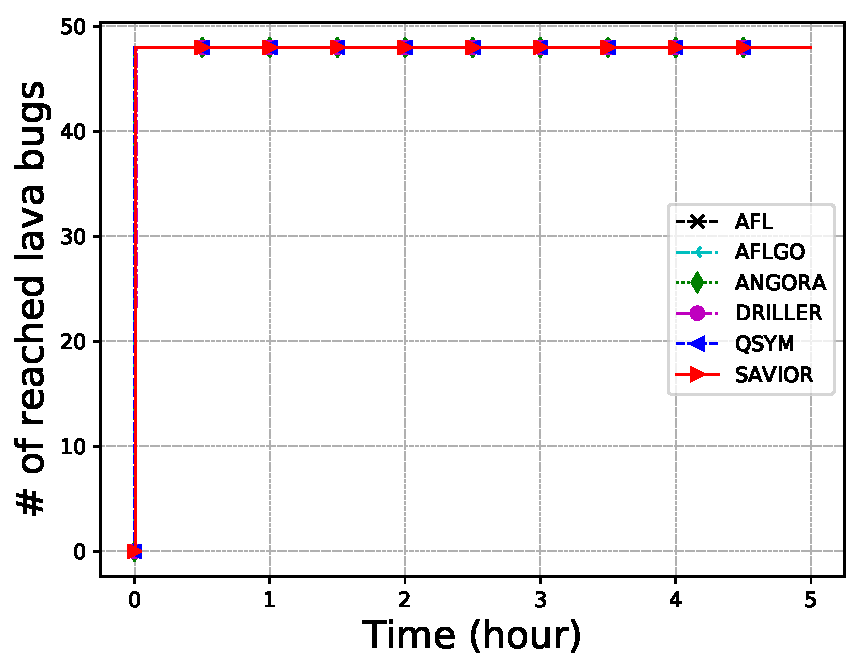
\includegraphics[width=1\textwidth]{savior/figures/lava_base64_bugcov.pdf}
        \caption{\scriptsize{Number of bugs reached in base64}}
        \label{fig:eval:lava:uniq}
    \end{subfigure}
        \begin{subfigure}[b]{0.24\textwidth}
        \centering
        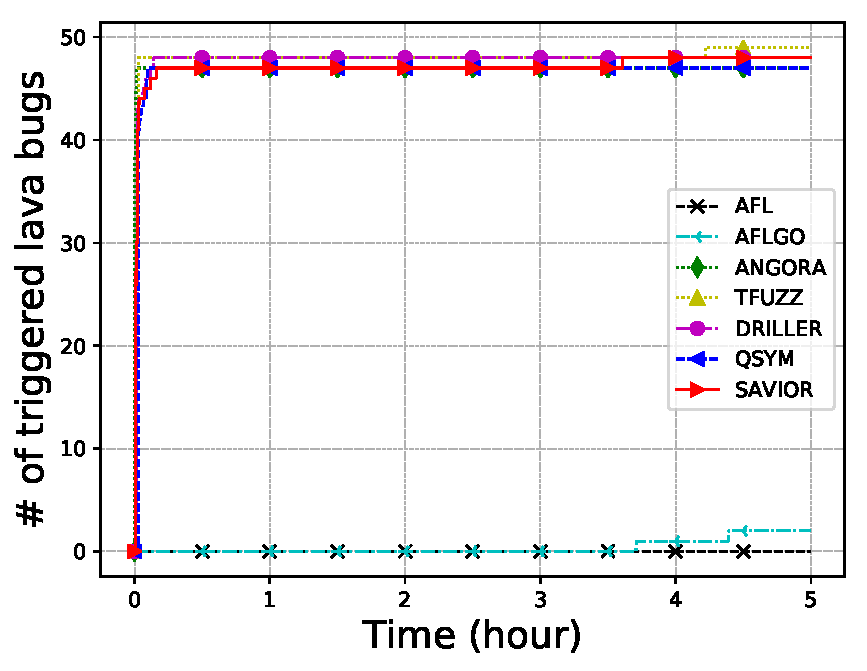
\includegraphics[width=1\textwidth]{savior/figures/lava_base64.pdf}
        \caption{\scriptsize{Number of bugs triggered in base64}}
        \label{fig:eval:lava:base64}
    \end{subfigure}\\
    \begin{subfigure}[b]{0.24\textwidth}
        \centering
        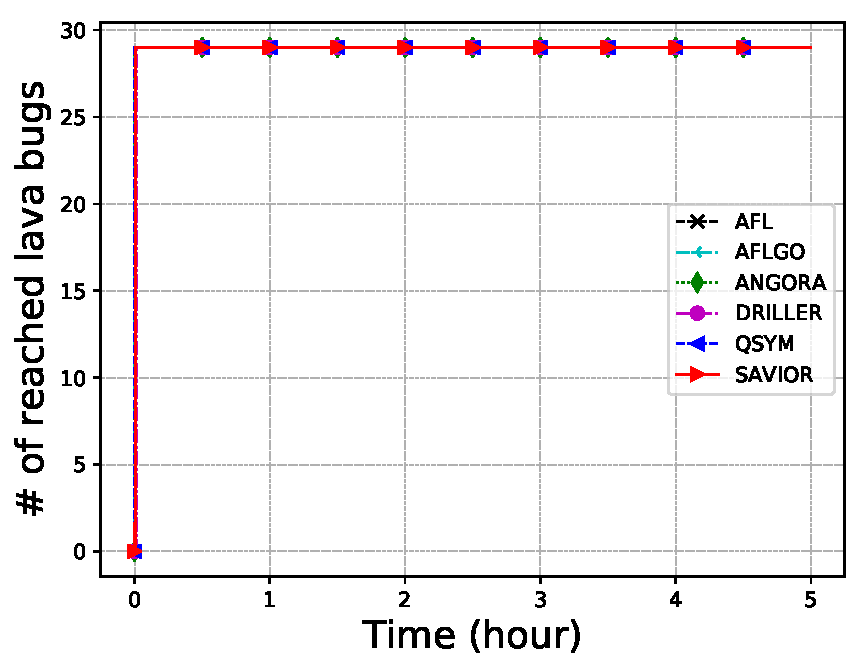
\includegraphics[width=1\textwidth]{savior/figures/lava_uniq_bugcov.pdf}
        \caption{\scriptsize{Number of bugs reached in uniq}}
        \label{fig:eval:lava:uniq}
    \end{subfigure}
    \begin{subfigure}[b]{0.24\textwidth}
        \centering
        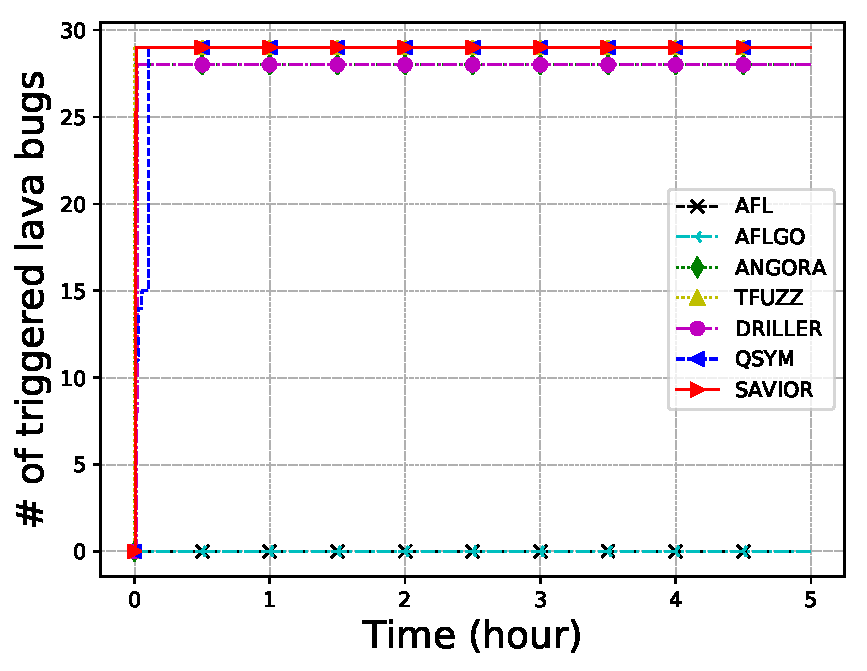
\includegraphics[width=1\textwidth]{savior/figures/lava_uniq.pdf}
        \caption{\scriptsize{Number of bugs triggered in uniq}}
        \label{fig:eval:lava:base64}
    \end{subfigure}\\
    \begin{subfigure}[b]{0.24\textwidth}
        \centering
        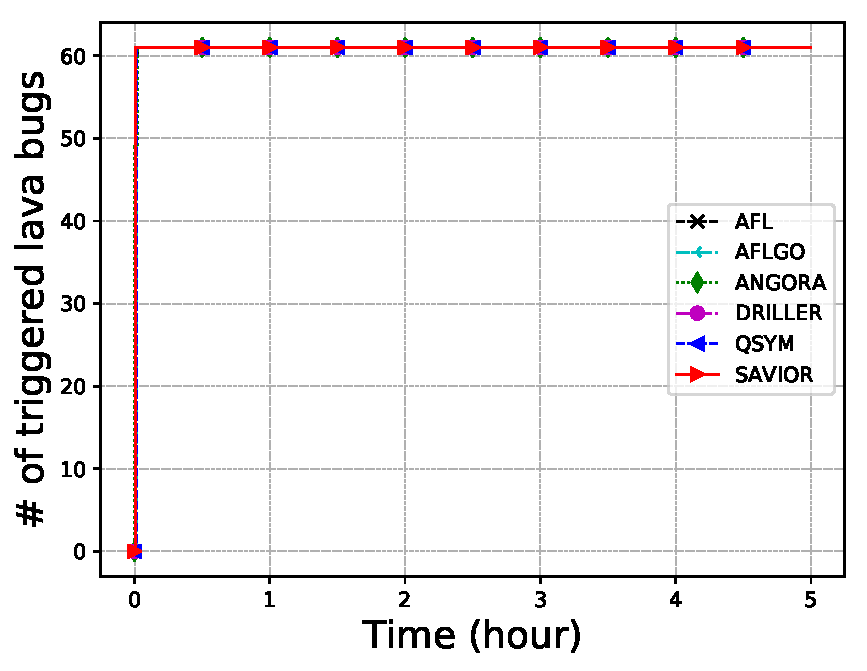
\includegraphics[width=1\textwidth]{savior/figures/lava_md5sum_bugcov.pdf}
        \caption{\scriptsize{Number of bugs reached in md5sum}}
        \label{fig:eval:lava:who}
    \end{subfigure}  
    \begin{subfigure}[b]{0.24\textwidth}
        \centering
        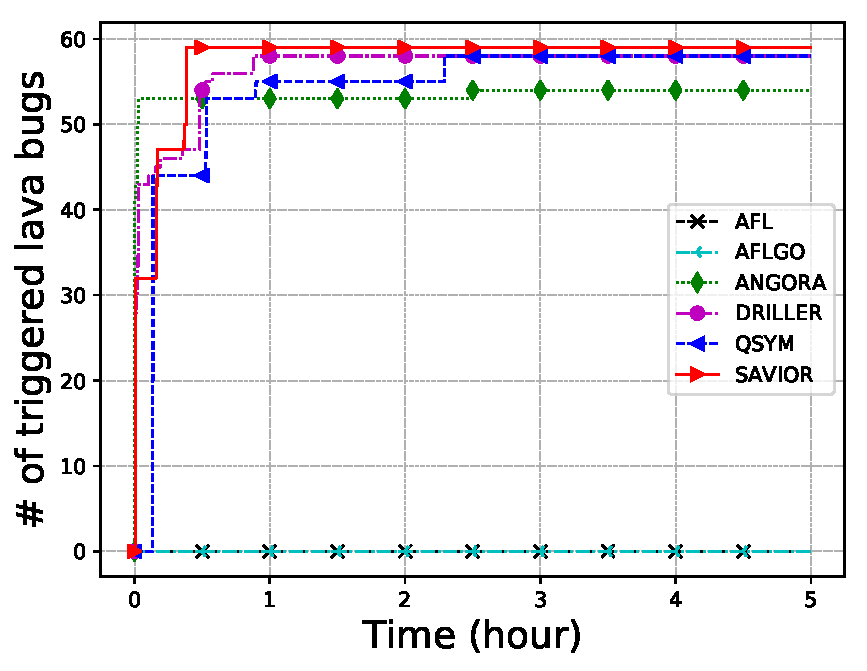
\includegraphics[width=1\textwidth]{savior/figures/lava_md5sum.pdf}
        \caption{\scriptsize{Number of bugs triggered in md5sum}}
        \label{fig:eval:lava:md5sum}
    \end{subfigure}\\
    \begin{subfigure}[b]{0.24\textwidth}
        \centering
        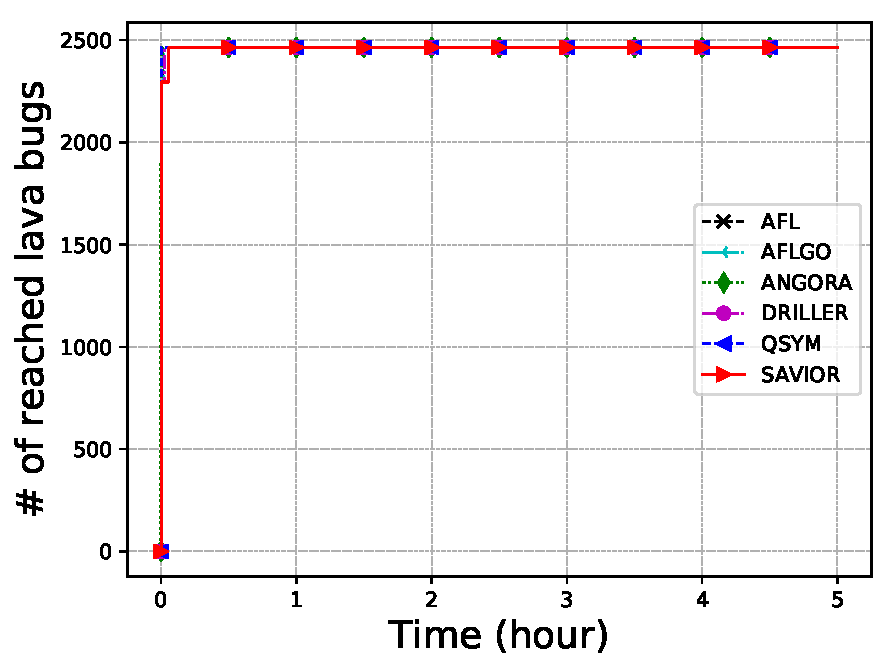
\includegraphics[width=1\textwidth]{savior/figures/lava_who_bugcov.pdf}
        \caption{\scriptsize{Number of bugs reached in who}}
        \label{fig:eval:lava:who}
    \end{subfigure}
    \begin{subfigure}[b]{0.24\textwidth}
        \centering
        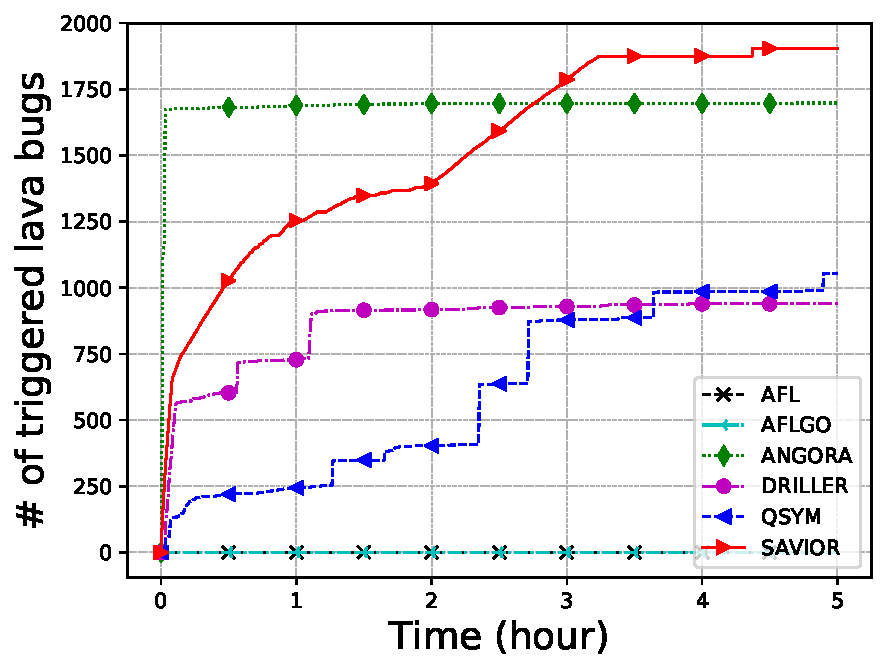
\includegraphics[width=1\textwidth]{savior/figures/lava_who.pdf}
        \caption{\scriptsize{Number of bugs triggered in who}}
        \label{fig:eval:lava:md5sum}
    \end{subfigure}
    \caption{Evaluation results with LAVA-M. The left column shows the number of reached lava-bugs by those fuzzers while the right column shows the number of lava-bug triggered by different fuzzers. For {\tt TFuzz}, we only present the number of triggered bugs in {\tt base64} and {\tt uniq}, as the other resutls are not reliable due to defects in a third-party component. This has been confirmed with the developers of {\tt TFuzz}.}
    \label{fig:lava_cfa}
\end{figure}





\subsection{Preliminary Results and Analysis}
\label{savior:sec:eval}

\subsubsection{Evaluation with LAVA-M}


\begin{table*}[h]
	\centering
		\caption{Fuzzer specific settings in evaluation with Lava-M.}
		\label{tab:lava-setup}
		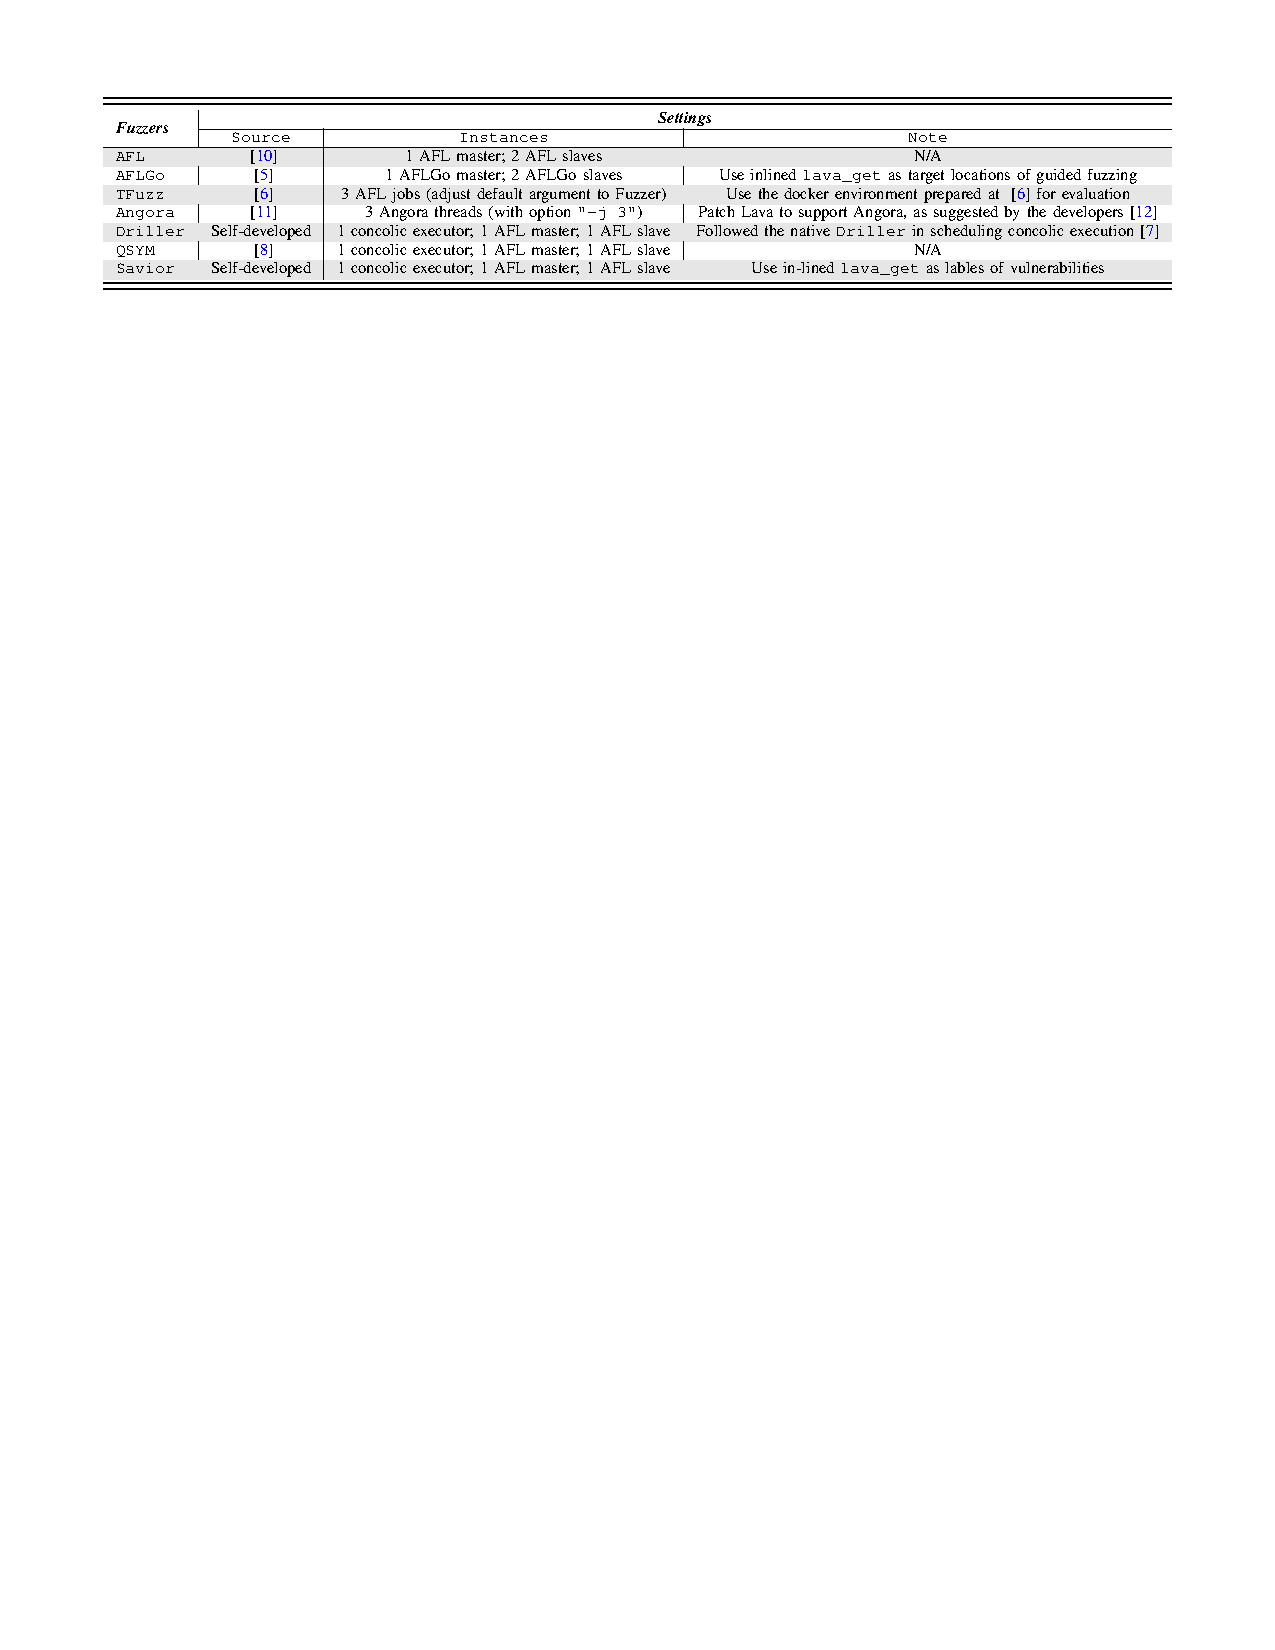
\includegraphics[scale=1]{savior/tables/lavasetup}
\end{table*}

\paragraph{Experimental Setup}
In this evaluation, we run each of the fuzzers in Table~\ref{tab:lava-setup} with four 
LAVA-M~\cite{lava} programs and we use the seeds shipped with the benchmark.  
For consistency, we conduct all the experiments on r4.16xlarge amazon EC2 instances 
with Ubuntu 16.04 LTS and we sequentially run all the experiments to avoid interference. 
In addition, we affiliate each fuzzer with 3 free CPU cores to ensure fairness with computation resources. 
Following the previous works~\cite{qsyminsu, angora,tfuzz}, we run each test for 5 hours.
To minimize the effect of randomness in fuzzing, we repeat each test 5 times and 
report the average results.
The settings specific to each fuzzer is summarized in Table~\ref{tab:lava-setup}, 
including how we distribute the 3 CPU cores and the actions we take to accommodate those fuzzers. 
In LAVA-M, each artificial vulnerability is enclosed in a function call to {\tt lava\_get} (in-lined in our evaluation).
We use these calls as the targets to guide {\tt AFLGo} and we mark them as vulnerability labels 
to enable bug-driven prioritization in \savior. In addition, as the vulnerability condition is 
hard-coded in the {\tt lava\_get} function, we naturally have support for bug-guided search.
Finally, for {\tt Angora}, we adopt the patches as suggested by the developers~\cite{tool-angora1}. 

\paragraph{Evaluation Results}In the left column of Figure~\ref{fig:lava_cfa}, 
we show how many vulnerabilities are reached over time by different fuzzers. The results demonstrate that all 
the fuzzers can instantly cover the code with LAVA vulnerabilities. However, as presented 
in the right column of Figure~\ref{fig:lava_cfa}, \tfuzz, \angora, \driller, \qsym, and \savior are able to 
trigger most (or all) of the vulnerabilities while \afl and \aflgo can trigger few. 
The reason behind is that the triggering conditions of LAVA vulnerabilities are all in the form of 
32-bit magic number matching. Mutation-based fuzzers, including AFL
and AFLGo, can hardly satisfy those conditions while the other fuzzers are all featured 
with techniques to solve them. 

Despite \tfuzz, \angora, \driller, \qsym, and \savior all trigger large numbers of LAVA vulnerabilities, 
they differ in terms of comprehensiveness and efficiency. \tfuzz quickly covers 
the listed vulnerabilities in {\tt base64} and {\tt uniq}. This is attributable to 
that (1) \tfuzz can reach all the vulnerabilities with the initial several seeds and (2) \tfuzz 
can transform the program to immediately trigger the encountered vulnerabilities.
Note that we do not show the results of \tfuzz on {\tt md5sum} and {\tt who},
because \tfuzz gets interrupted by a defective third-party component\footnote{This has been confirmed with the 
developers.}. For all the cases, \angora triggers most vulnerabilities
immediately after its start. The main reason is that the ``black-box function'' 
pertaining to all LAVA vulnerabilities 
is {\tt f(x) = x} and the triggering conditions are like {\tt f(x) == CONSTANT}. 
\angora always starts evaluates such functions with {\tt x = CONSTANT} and therefore, 
it can instantly generate seeds that satisfy the vulnerability conditions. 
In the case of {\tt who}, \angora does not make all the vulnerabilities 
because of the incomplete dynamic taint analysis. 

Regarding the three hybrid tools, they can trigger every vulnerability 
that their concolic executor encounters. In the cases of {\tt base64}, {\tt uniq}, and {\tt md5sum}, 
their concolic executor can reach all the vulnerabilities with (arbitrary) initial seeds,
which explains why the fuzzers all quickly trigger the listed vulnerabilities (regardless of their seed scheduling). 
But in the case of {\tt who}, even though the fuzzing component quickly generate
seeds to cover code containing vulnerabilities, 
it takes the concolic executor much longer to run those seeds.
For instance, while executing the inputs from \afl, \qsym needs 
around 72 hours of continuous concolic execution to reach 
all the LAVA vulnerabilities in {\tt who}. It's worth noting that \driller (with a random seed scheduling) 
moves faster than \qsym, because \qsym prioritizes concolic execution 
on small seeds, while reaching many vulnerabilities in {\tt who} needs larger seeds.

\begin{table*}[h]
	\centering
	\begin{minipage}[b]{0.45\textwidth}
		\centering	
		\caption{Bug triggered by different fuzzers in evaluation with Lava-M (with bug-guided search).}
		\label{tab:lava-bug-num}
		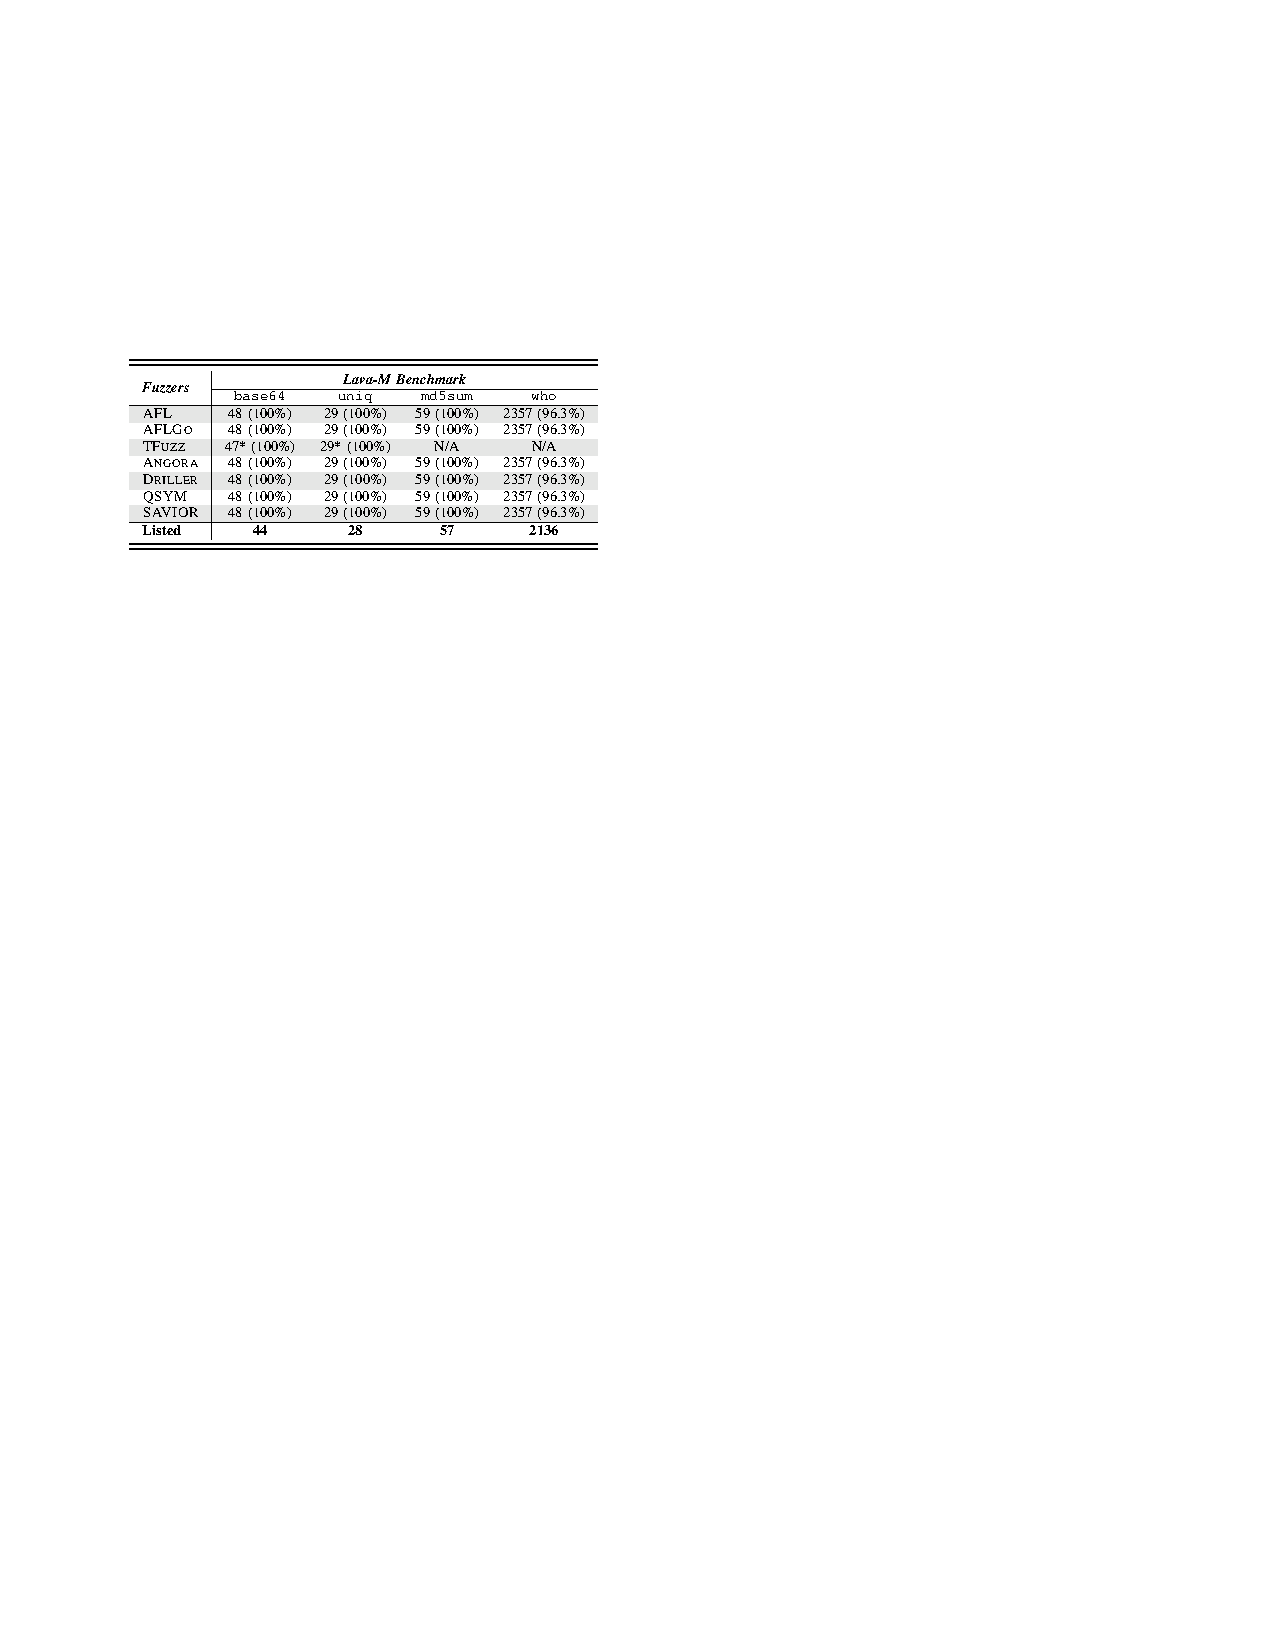
\includegraphics[scale=0.80]{savior/tables/bugguidedsearchlava}
	\end{minipage}
 	\hfill
	\begin{minipage}[b]{0.45\textwidth}
		\centering	
		\caption{IDs of Lava bugs that are not listed but identified by bug-guided search.}
		\label{tab:new-laval-bug-search}
		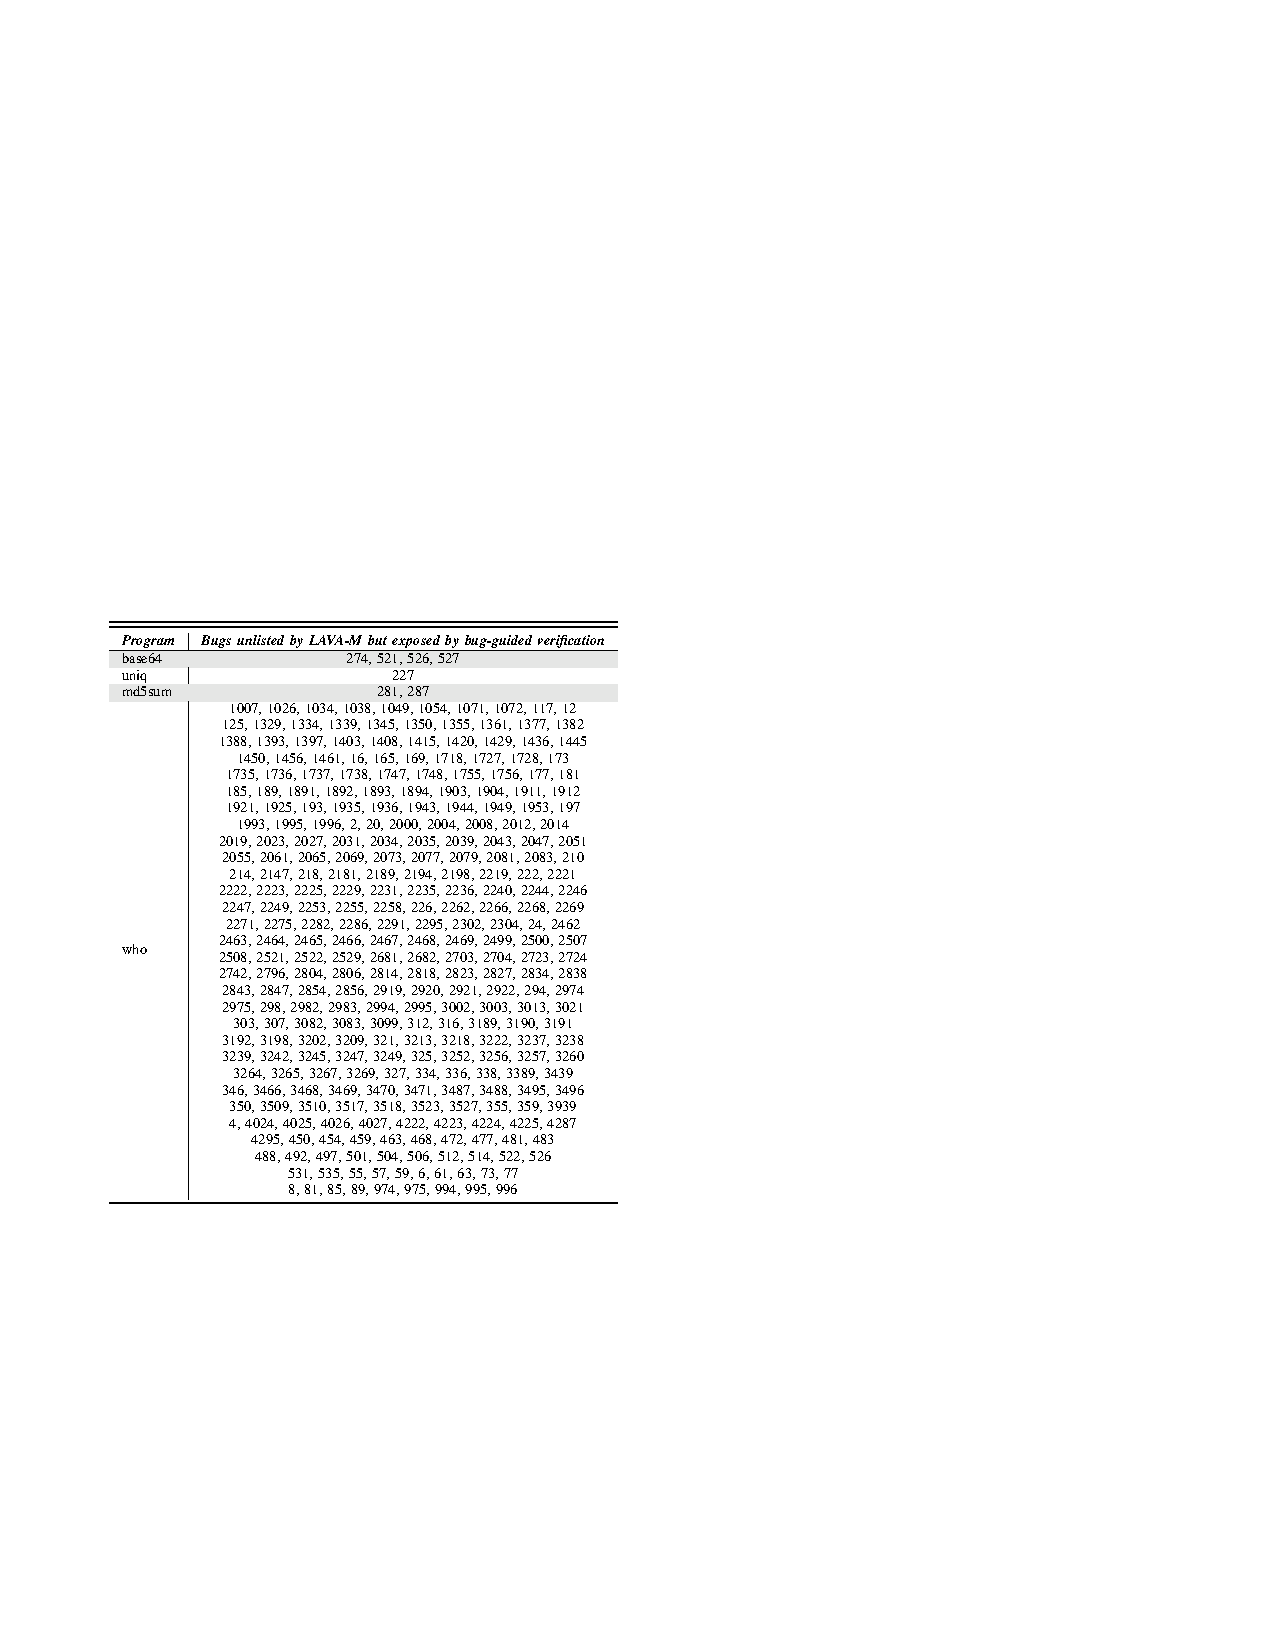
\includegraphics[scale=0.80]{savior/tables/unlistedlavabug}
	\end{minipage}
\end{table*}


As mentioned before, all the fuzzers have generated seeds to reach all the vulnerabilities, which they cannot 
trigger all of them either because their incapability to satisfy the conditions or because they did not finish 
concolic execution on all the seeds. We extended a further experiment by performing bug-guided searching with 
the seeds from all the fuzzers. Simply speaking, we run each of the seeds from all the fuzzers with the 
concolic executor in \savior. In this experiment, we only do constraint solving when a LAVA-M vulnerability condition
is encountered. This simulates the process of bug-guided search for all fuzzers. Enhanced with our bug-guided search, all the fuzzers 
can trigger not only the listed bugs in LAVA, as shown in Table~\ref{tab:lava-bug-num}, 
but also a group of unlisted bugs (Table~\ref{tab:new-laval-bug-search}). 








